\section{Introduction}

\subsection{World Full of Graphs}\label{ss_11}

Graphs are a natural way to describe complex interactions between entities. We use graphs/networks interchangeably in the notes, though graph is a more commonly seen in mathematical settings defined as $G(V, E)$.

Common networks include human society, chemical interactions, connection of neurons, knowledge graphs, etc. You can roughly separate those into (1) naturally defined (2) man-made, but the distinction is often difficult. As we will be discussing in later chapters, network relationships using traditional methods. We use \textit{spectral clustering}\ref{?} to extract community association; \textit{pagerank} to trace flow of trust; \textit{message propagation} for probabilistic inference. In addition, we will also introduce the recently booming field of \textit{graph neural networks}, whose effectiveness in understanding rich relational structure have been demonstrated by researchers.

\begin{figure}[ht]
  \centering
  \begin{subfigure}{0.45\textwidth}
    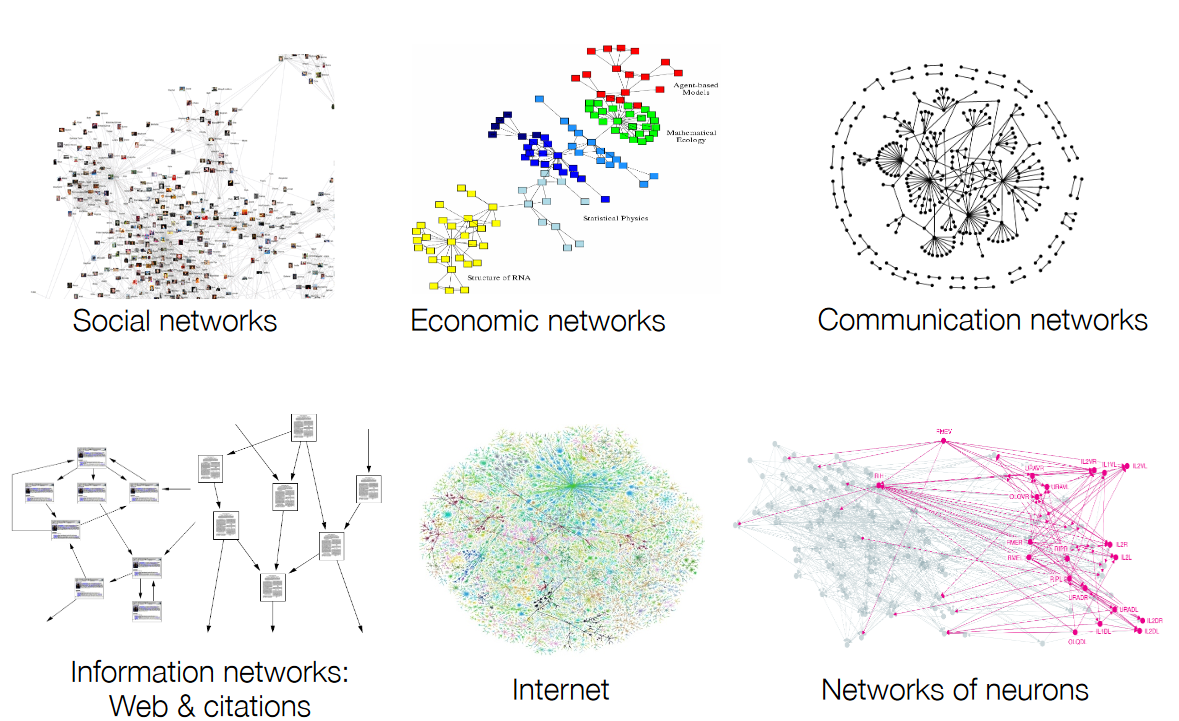
\includegraphics[width=\textwidth]{img/l1_p7_networks1.PNG}
    \caption{Lecture 1, Page 7}
    \label{fig:1}
  \end{subfigure}
  %
  \begin{subfigure}{0.45\textwidth}
    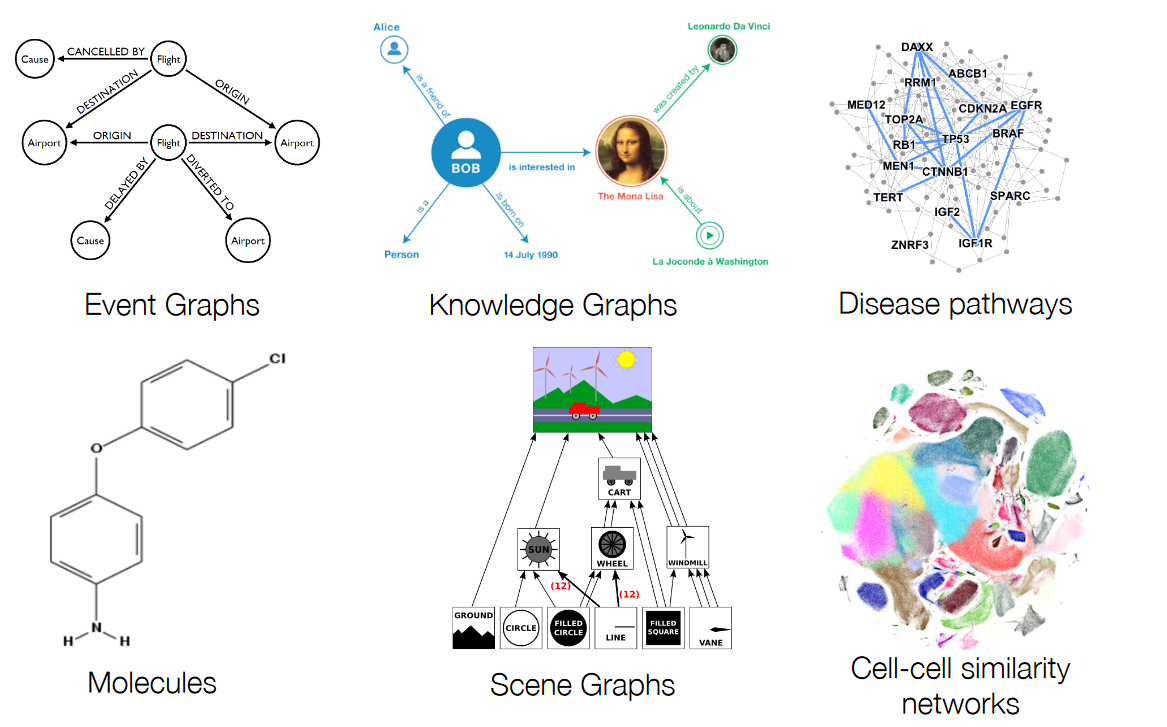
\includegraphics[width=\textwidth]{img/l1_p10_networks2.PNG}
    \caption{Lecture 1, Page 10}
    \label{fig:2}
  \end{subfigure}
\end{figure}

\subsection{Real World Application of Graphs}

In general, our analysis of a network fall in the following categories:

\begin{itemize}
    \item \textit{Node classification}: Predict the type of a given node
    
    \item \textit{Link prediction}: Predict the interaction (or existence of) between two nodes
    
    \item \textit{Community detection}: Identify linked clusters of nodes
    
    \item \textit{Network similarity}: Measure similarity among nodes/sub-graphs/whole networks
\end{itemize}

\subsubsection{Social Network}

We were used to be told there is 6-degree of separation. Researchers found in 2012 \href{https://web.stanford.edu/~jugander/papers/websci12-fourdegrees.pdf}{[link]} that according to social graph built from Facebook data, average distance between people is in fact $3.74$, much less than $4.4 - 5.7$ range discovered in 1967 \href{shorturl.at/gCMSU}{[link]} as the famous ``The Small World Problem".

{
\centering
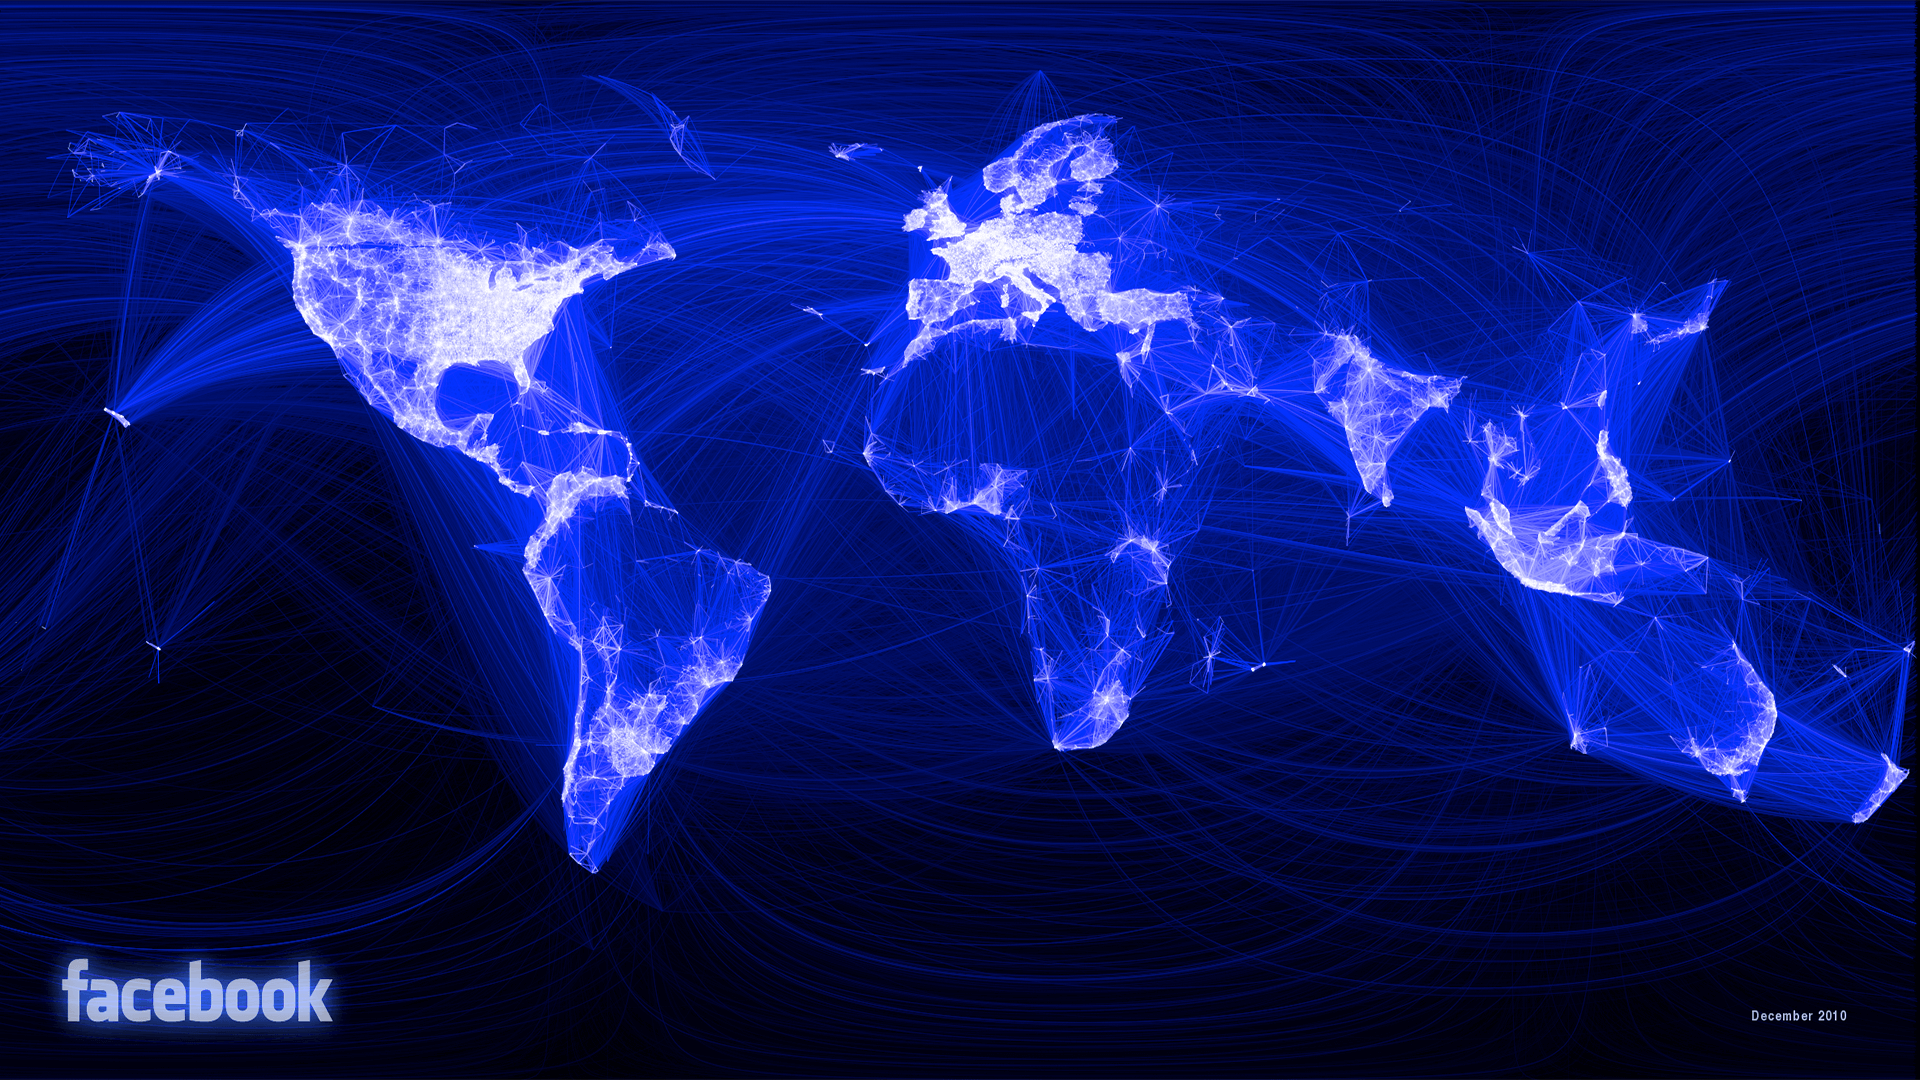
\includegraphics[width=0.75\linewidth]{img/n1_fb.png} \par
}

With clustering techniques we can also discover social circles. On the right is sample image extracted from a method \href{https://cs.stanford.edu/people/jure/pubs/circles-nips12.pdf}{[link]} to identify social circles using network structure and user profiles.

{
\centering
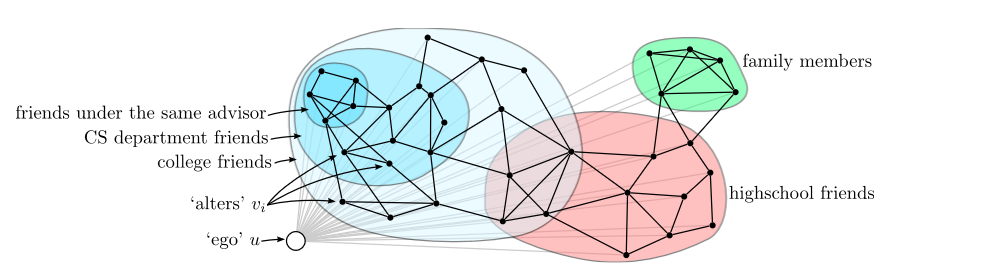
\includegraphics[width=0.85\linewidth]{img/n1_social.png} \par
}

We can separate the re-tweet network along party lines  using techniques similar to social circle detection. Explanation for the image below is \href{https://qz.com/1024117/one-visualization-shows-how-morally-outraged-tweets-stay-within-their-political-bubble/}{[here]}.

{
\centering
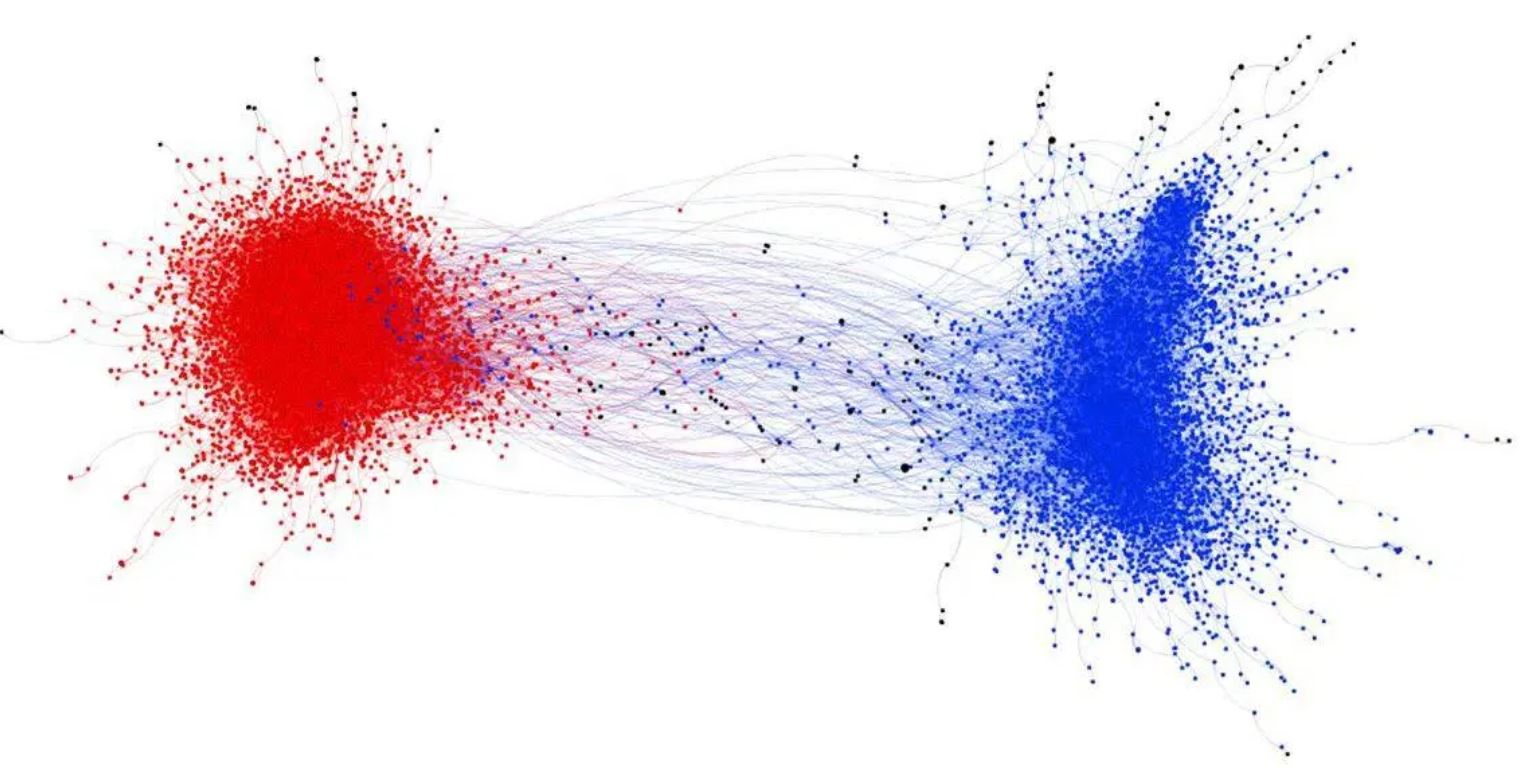
\includegraphics[width=0.6\linewidth]{img/n1_twitter.jpg} \par
}


\subsubsection{Influence Propagation}

Network analysis is also useful for identifying weaknesses in infrastructure network. Below shows a blackout happened on August 15, 2003 (August 14 vs August 15), affecting much of the East Coast, affecting Canadian and American cities alike. Notice how Toronto/Detroid are completely gone and DC - Boston corridor is significantly dimmer. Higher resolution image \href{https://earthobservatory.nasa.gov/images/3719/blackout-leaves-american-cities-in-the-dark}{[here]}. With network analysis tools, we can find out which nodes (cities) will be affected, severity of the impact and speed of the spread. 

{
\centering
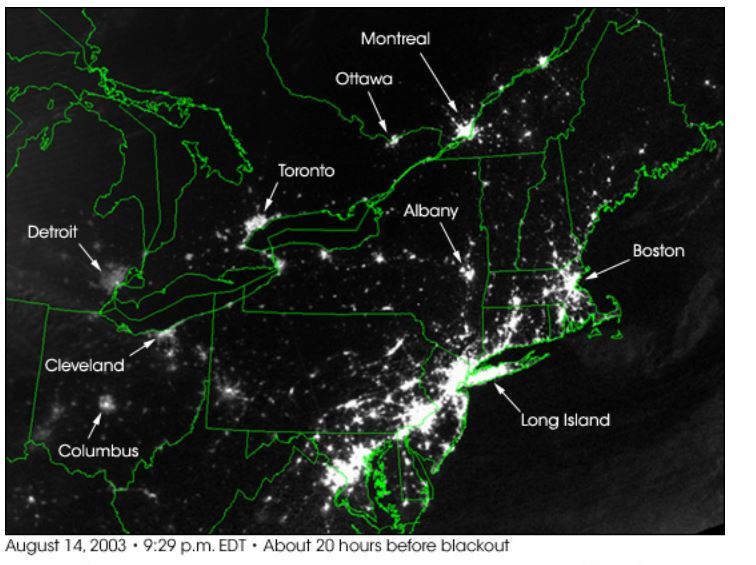
\includegraphics[width=0.45\linewidth]{img/n1_blackout.jpg}
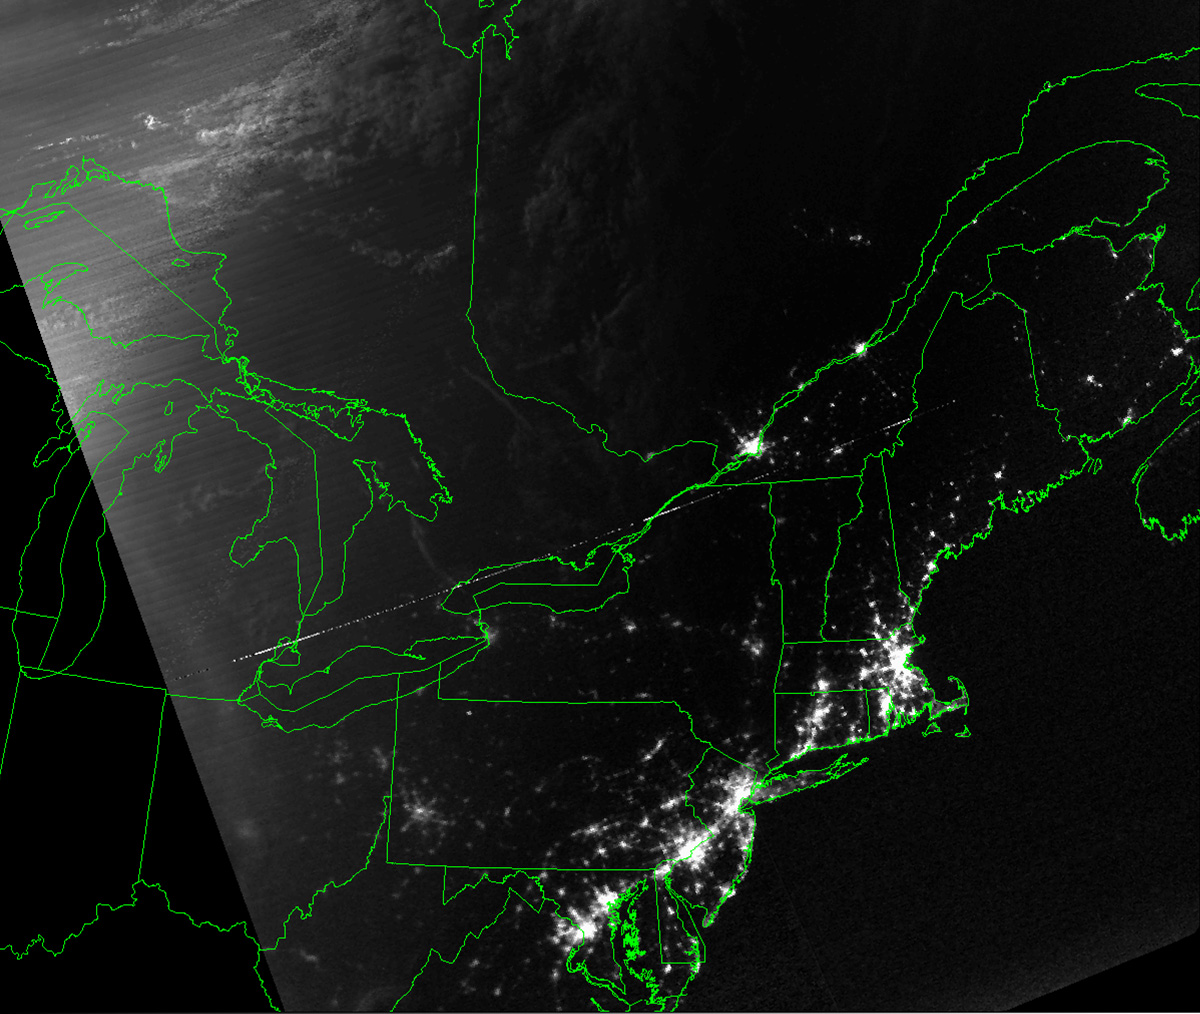
\includegraphics[width=0.45\linewidth]{img/n1_blackout2.jpg}\par
}

This failure propagation model is also applicable for spread for mis-information and spread of virus. With a virus spread model, you are modeling connectivity (probability of disease spread) between people, community, city and countries. Identifying and cutting off center of spread can localize the effect of disease spread. See CDC's model on pandemic influenza published back in 2006 \href{https://wwwnc.cdc.gov/eid/article/12/11/06-0255-f4}{[here]}.

{
\centering
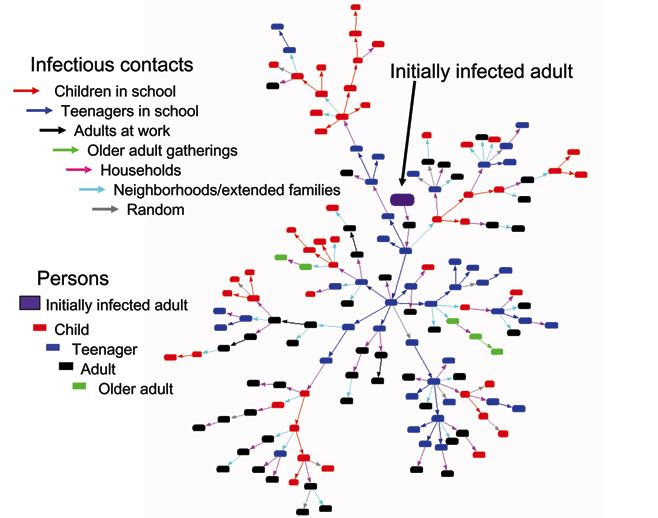
\includegraphics[width=0.6\linewidth]{img/n1_virus.jpg}\par
}

\subsubsection{Knowledge Graph}

Knowledge graph is a great example of heterogeneous graph, graphs that contain nodes with different meanings. Typically in a knowledge graph, there are item nodes and property/category nodes. 

{
\centering
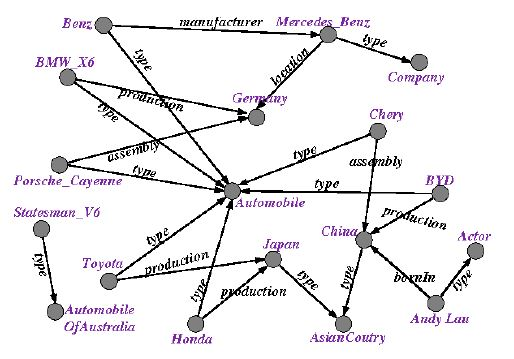
\includegraphics[width=0.32\linewidth]{img/l1_p22_1.jpg}
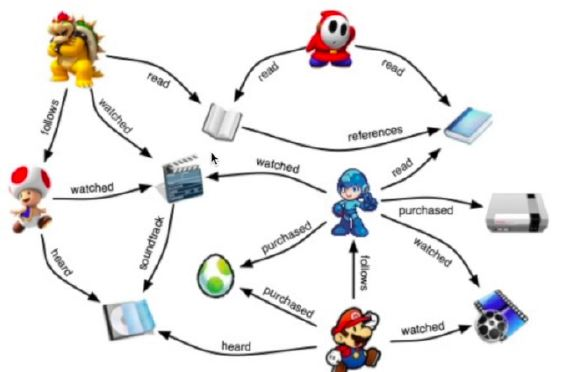
\includegraphics[width=0.32\linewidth]{img/l1_p22_2.jpg}
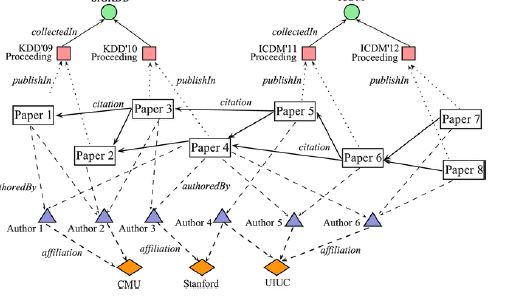
\includegraphics[width=0.32\linewidth]{img/l1_p22_3.jpg}\par
}

\subsubsection{Recommender System}

Predicting user preference can be abstracted to predicting existence of edges in a bipartite graph. CS246 covered concepts like SVD (singular value decomposition), but you can also solve this by treating user preference matrix as an adjacency matrix. In class, we showed that Pinterest has its own image-embedding based graph search algorithm, handling 300 million users, more than 4 billion pins and more than 2 billion boards. Notice that Pinterest is building a ``tri-partite" graph with user, pins and boards.

{
\centering
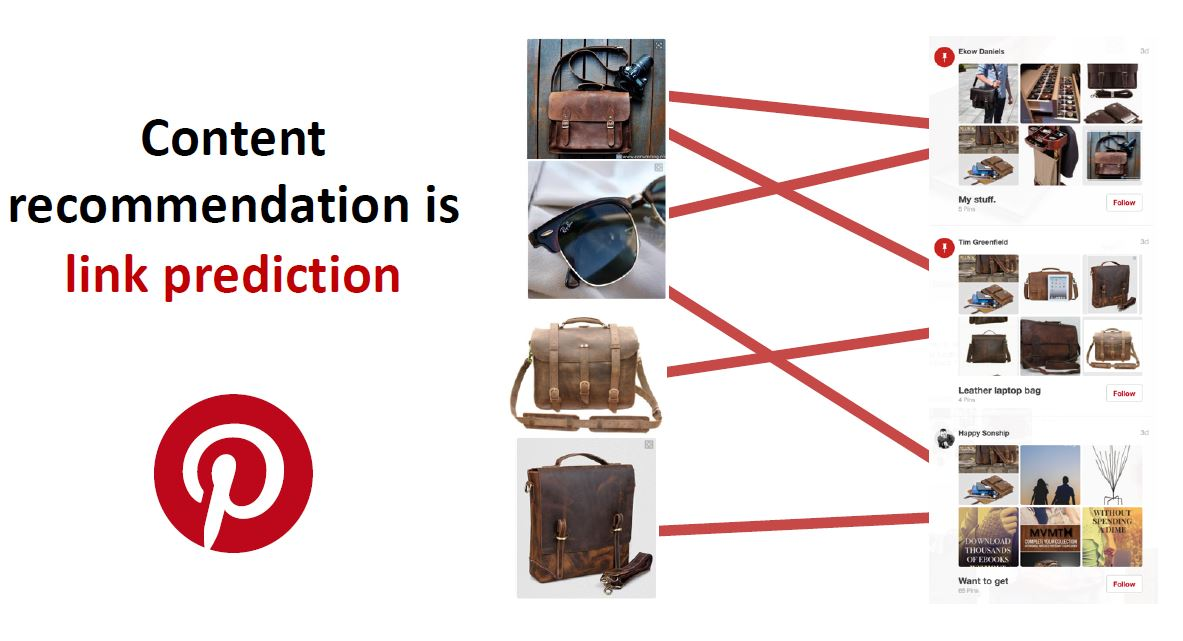
\includegraphics[width=0.5\linewidth]{img/l1_p24.jpg}\par
}

It is not un-common to combine recommender system's bi-partite graph with an underlying knowledge graph. An obvious use case is movie recommendation, where movies have attributes like genre, theme, director, actor/actress, etc. This can be treated as an overlay of multiple disjoint graphs, but the fully combined graph has the best predictive power \href{https://www.kdd.org/kdd2016/papers/files/adf0066-zhangA.pdf}{[link]}.

{
\centering
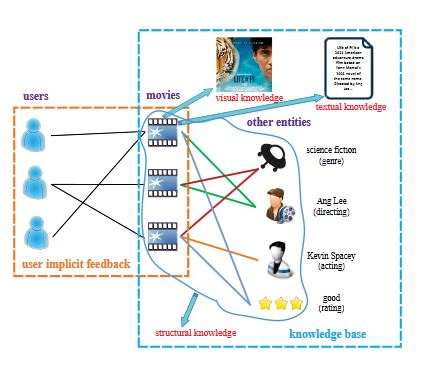
\includegraphics[width=0.5\linewidth]{img/n1_movies.jpg}\par
}


\subsubsection{Biochemical Applications}

Biological pathways, ``network" derived from atomic structure of drugs and proteins, interaction/effect/side effect of drugs and even the food chain naturally form networks with potentially heterogeneous nodes. Using Graph Convolutional Networks \label{??} to predict effect of chemicals has gained traction in recent years to compete with point-cloud based, 3D voxel convolution techniques. For example, effect of drug combinations can be modeled using a heterogeneous graph with nodes representing drug and protein \href{https://www.kurzweilai.net/how-to-predict-the-side-effects-of-millions-of-drug-combinations}{[link]}.

{
\centering
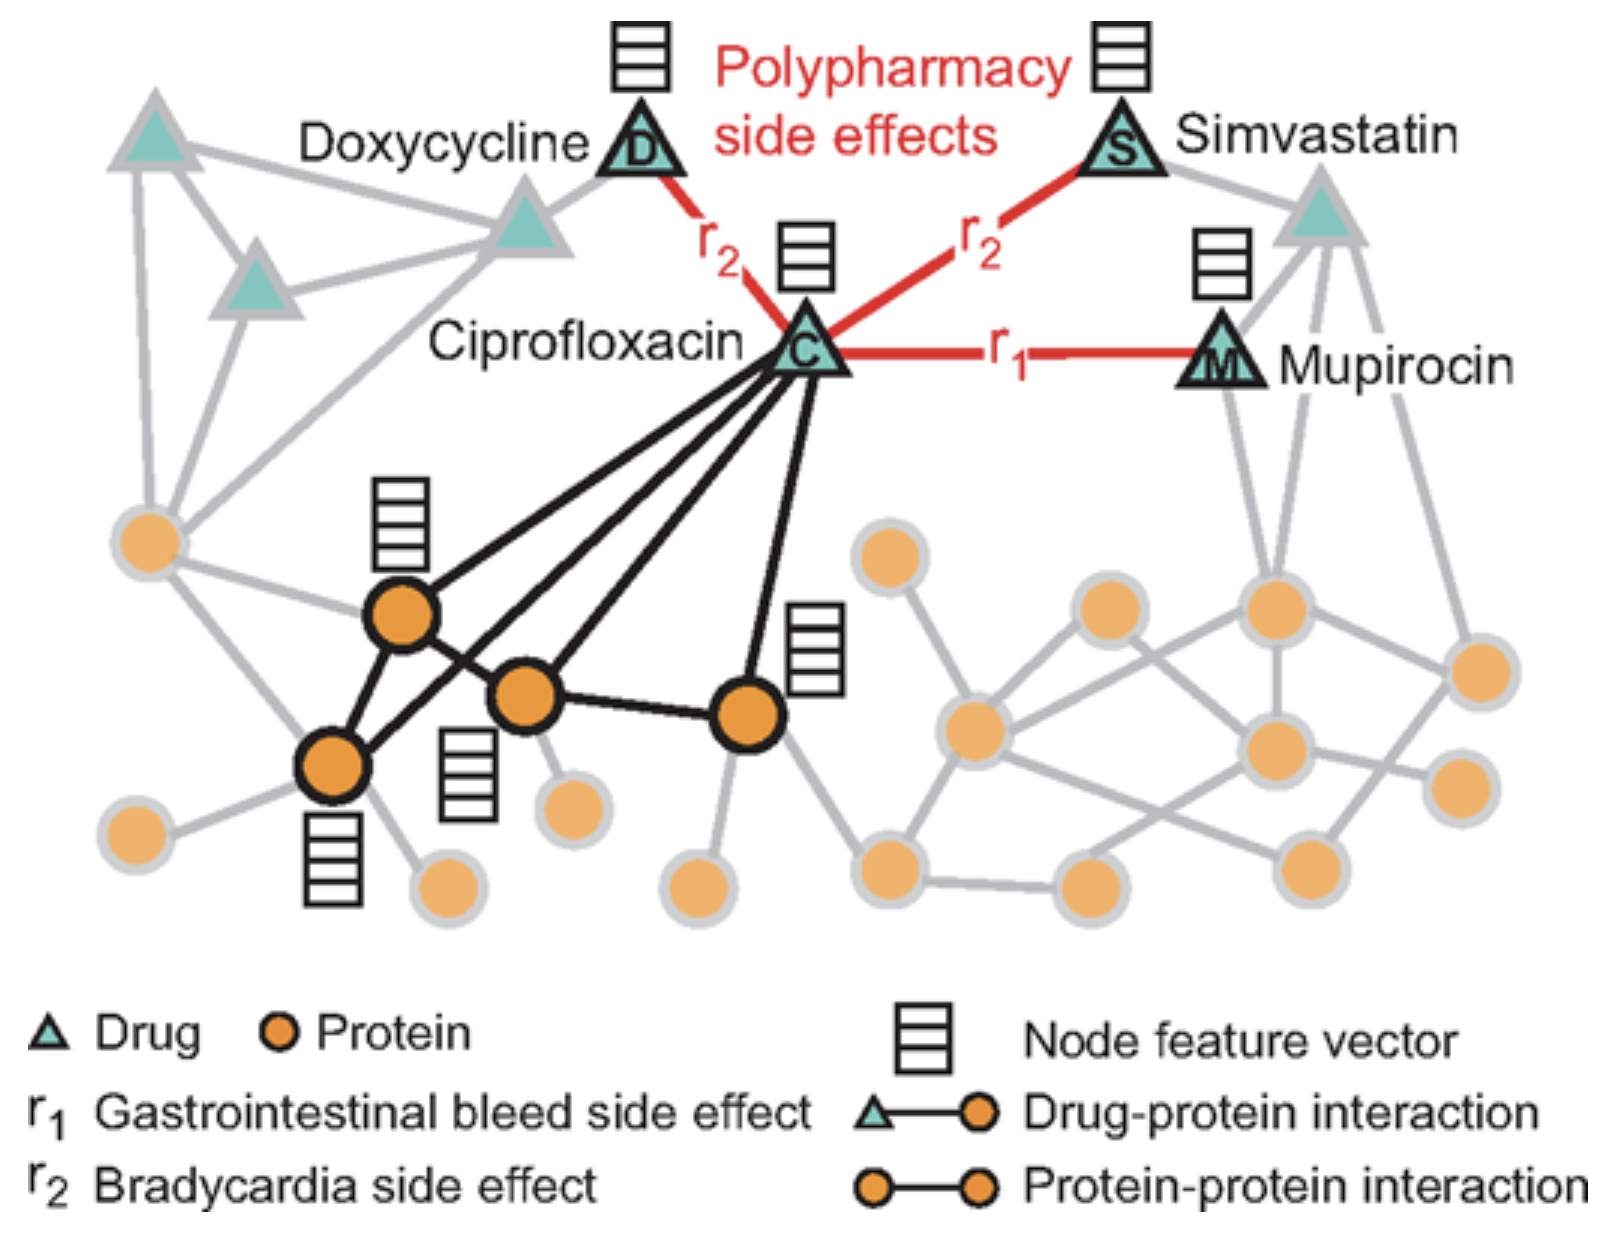
\includegraphics[width=0.5\linewidth]{img/n1_drug.png}\par
}